% Cover letter using letter.sty
\documentclass[]{letter} % Uses 10pt
%\documentstyle[newcent]{letter}
\usepackage{pdfpages}
%Use \documentstyle[newcent]{letter} for New Century Schoolbook postscript font
% the following commands control the margins:
\topmargin=-1in    % Make letterhead start about 1 inch from top of page 
\textheight=8in    % text height can be bigger for a longer letter
\oddsidemargin=0pt % leftmargin is 1 inch
\textwidth=6.5in   % textwidth of 6.5in leaves 1 inch for right margin

\begin{document}

%\signature{Daniel M. Topa}                % name for signature 
\longindentation=0pt                       % needed to get closing flush left
\let\raggedleft\raggedright                % needed to get date flush left
 
\begin{letter}{\emph{Journal of Approximation Theory} \\
Paul Nevai, Editor-in-Chief\\Amos Ron, Editor-in-Chief}

\begin{flushleft}
{\large\bf Engility Corporation\\}
{\large\bf USACE Engineer Research and Development Center}
\end{flushleft}
\medskip\hrule height 1pt
%\begin{flushright}
%\hfill X Division \\
%\hfill POB 1663 \\
%\hfill Los Alamos NM 87545 \\
%\end{flushright} 
\vfill % forces letterhead to top of page

 
\opening{Kind Sirs,} %  .  .  .  .  .  .  .  .  .  .  .  .  .  .  .  .  .  .  .  .  .  .  .  .  .  .  .  .
 
\noindent The goal of our paper \emph{Surprising Homotopies in the Zernike basis} is to extend the tools of Fourier analysis to the disk polynomials of Zernike which can be viewed as a Fourier basis with polynomial weighting. Zernike's polynomials are the appropriate set when the domain is the unit disk making them appropriate to optical physicists dealing with round apertures and components. Zernike and his student Nijboer connected these functions to the Seidel aberrations making the disk polynomials a standard in aberration theory. The Zernike polynomials are enjoying a Renaissance driven by their introduction into optometry and ophthalmology and their prevalence grows.

\noindent This research project culminated from two different efforts: extending phase front measurements beyond paraxial approximations and resolution of point-like aberrations which involved examination of phase fronts for point sources (sphere) and inertial sources (cone). The approximations for the sphere and the cone have the exact same magnitudes in the Zernike basis.
The deep connection between these different surfaces was startling. Attempting to resolve this relationship lead us to explore the tools of approximation theory; the results are described in detail in the paper.

\noindent Allow me to address the issues raised in your FAQ web page.

\begin{enumerate}
\item Specify special considerations that should be given to the paper. \emph{No special considerations requested.} \\

\item A brief background regarding the research involved or how the data was collected. \emph{This effort was born at the confluence of two independent investigations: applying tools from Fourier analysis to Zernike decompositions and the approximation of point aberrations in polynomial representations.} \\

\item The Author to whom we should address our correspondence. \emph{Daniel Topa.} \\

\item A contact address, telephone/fax numbers and e-mail address.  \emph{Included in signature block.} \\

\item Details of any previous or concurrent submissions.  \emph{Previous submission as ACHA-14-13; no concurrent submissions.} \\

\item It is also useful to provide the Editor-in-Chief with any information that will support your submission.  \emph{A series \emph{Mathematica} notebooks demonstrates the validity of the computations with explicit examples.} \\

\item The inclusion (or exclusion) of certain Reviewers. When providing the names of potential Reviewers, please supply their full contact details including an e-mail address.  \emph{No preferences for reviewers.} \\
\end{enumerate}


\noindent Thank you for your attention.
\\

Sincerely, \\
\\
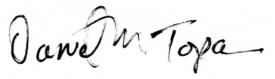
\includegraphics[]{signature001}\\
Daniel M. Topa \\
POB 82-1002 \\
Vicksburg, MS 39182-1002 \\
(505) 504-5986 
%\closing{Sincerely,}
\end{letter}
  
%\includepdf[pages={1-7}]{../"Mathematica verification".pdf}

\end{document}






